\section{Introduction to Compilers}
Some examples of compilers we've used in this class include 
\begin{center}
    \begin{tabular}{|c|c|}
        \hline 
        \code{gcc} & C to binary  \\ 
        \code{g++} & C++ to binary  \\ 
        \code{rustc} & Rust to binary \\ 
        \code{javac} & Java to JVM bytecode \\ 
        \code{ghc} & Haskell to Haskell magic \\ 
        \code{tsc} & TypeScript to JavaScript \\ 
        \hline 
    \end{tabular}
\end{center}
Essentially, a compiler takes some program and produces an output program, one that is easier for us to run in some environment. In this course, we're going to create a compiler \code{ucsdc} that takes in \code{snek} files and will produce \code{x86\_64} binaries.

\bigskip 

To be more specific, our compiler should do the following: given a \code{.snek} text file, 
\begin{itemize}
    \item parse\footnote{Known to be very boring.} the text into an abstract syntax tree (AST), 
    \begin{mdframed}
        (Example.) For example, consider the following Java class. 
\begin{verbatim}
class Pt {
    int x; 
    int y; 
}\end{verbatim}
        Its AST representation might look like 
        \begin{center}
            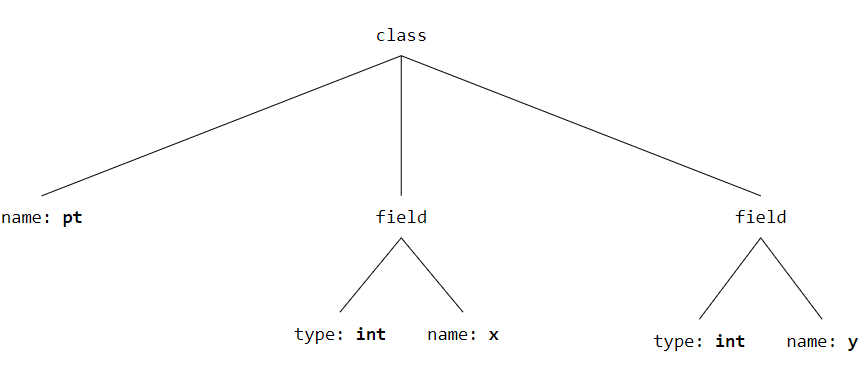
\includegraphics[scale=0.8]{assets/ast.png}
        \end{center}
    \end{mdframed}
    \item and either 
    \begin{itemize}
        \item generates assembly (or some other output program), or 
        \item generate an error message.
    \end{itemize}
\end{itemize}
We are \underline{not} interested in generating the most optimized assembly, just that it works. Most of the time spent in this course will be on the code generating part (i.e., from AST to assembly). Towards the \emph{end} of the course, we'll work with libraries/runtime.

\subsection{S-Expressions}
We'll be using s-expressions to represent our program's source code. That is, each \code{snek} file will contain s-expressions. S-expressions are defined as either 
\begin{itemize}
    \item An \textbf{atom} of the form $x$, or 
    \item An \textbf{expression} of the form $(x \quad y)$, where $x$ and $y$ are s-expressions. 
\end{itemize}
For example, \code{(sub1 2)} is an expression with two atoms, \code{sub1} and \code{2}. 

\subsubsection{The \code{sexp} Crate}
Most programming language will have a parser for s-expressions. In Rust, we have the \code{sexp} crate. This crate has the following \code{enum}s\footnote{In Rust, \code{enum}s are algebraic data types.}:
\begin{itemize}
    \item A \code{Sexp} enum, representing either an \code{Atom} or a vector of s-expressions. Vectors of s-expressions will contain two elements (since an expression has the form $(x \quad y)$, which has two expressions). 
    \begin{verbatim}
pub enum Sexp {
    Atom(Atom),
    List(Vec<Sexp>),
}
    \end{verbatim}

    \item An \code{Atom} enum, representing one of three different types of atoms: a \code{String}, \code{i64} (64-bit signed integer), or \code{f64} (double-precision float). 
    \begin{verbatim}
pub enum Atom {
    S(String),
    I(i64),
    F(f64)
}\end{verbatim}
\end{itemize}

\begin{mdframed}
    (Exercise.) Why is \code{Vec<Box<Sexp>>} or \code{Box<Vec<Sexp>>} not used in the \code{enum} definitions above? 

    \begin{mdframed}
        Remember that the reason why something like 
        \begin{verbatim}
enum Expr {
    Num(i32),
    Add1(Expr),
    Sub1(Expr)
}\end{verbatim}
        wouldn't work is because \code{Expr}, as a recursive type, could have infinite size. That is, we could nest \emph{many} \code{Expr}s, and since this value could theoretically continue infinitely, so we don't know how much space this recursive type needs. However, \code{Box<T>} is a pointer type that allocates memory on the heap. \code{Box<T>} has a \emph{fixed} size, so Rust is fine if we have \code{Box<Expr>}. 

        \bigskip

        The reason why we \emph{don't} need \code{Vec<Box<Sexpr>>} or \code{Box<Vec<Sexpr>>} in the above \code{enum}s is because \code{Vec<T>} allocates to the heap (when you add any elements; a vector created initially with no elements does not allocate). In other words, think of \code{Vec<T>} as being a resizable \code{Box<T>}. More accurately, a \code{Vec<T>} is a fixed-size type with a reference to variable-sized heap data.
    \end{mdframed}
\end{mdframed}


\begin{mdframed}
    (Exercise.) Represent the following s-expression in Rust: 
    \begin{verbatim}
        (sub1 (sub1 (add1 73)))\end{verbatim}
    
    \begin{mdframed}
        First, the s-expression itself is roughly similar to a tree, where each \emph{atom} is a leaf node and each \emph{list} is another s-expression. In any case, we can roughly structure the above s-expression like so: 
        \begin{verbatim}
(               // List
    sub1            // Atom 
    (               // List 
        sub1            // Atom 
        (               // List 
            add1            // Atom 
            73              // Atom 
        )
    )
) \end{verbatim}
        In other words, we have a list whose elements are an \emph{atom} and another \emph{list}. With this in mind, the Rust form is
        \begin{verbatim}
List(vec![
    Atom(S("sub1")),
    List(vec![
        Atom(S("sub1")),
        List(vec![
            Atom(S("add1")),
            Atom(I(73))
        ])
    ])
])\end{verbatim}
    \end{mdframed}
\end{mdframed}

\subsection{From S-Expressions to Rust Code}
Given some s-expression string, we can use the above crate to convert the s-expression into a Rust object. However, this Rust object itself doesn't give us much information aside from how the s-expression is structured. We want to turn this Rust object into another Rust object representing the actual expressions (i.e., an abstract syntax tree). We can use the Rust structure to represent our code: 
\begin{verbatim}
enum Expr {
    Num(i32),
    Add1(Box<Expr>),
    Sub1(Box<Expr>),
}\end{verbatim}
So, given the \code{Sexp}, our s-expression representation in Rust, we can use the following function to parse this representation into an abstract syntax tree: 
\begin{verbatim}
fn parse_expr(s : &Sexp) -> Expr {
    match s {
        Sexp::Atom(I(n)) =>
            Expr::Num(i32::try_from(*n).unwrap()),
            Sexp::List(vec) =>
                match &vec[..] {
                    [Sexp::Atom(S(op)), e] if op == "add1" =>
                        Expr::Add1(Box::new(parse_expr(e))),
                    [Sexp::Atom(S(op)), e] if op == "sub1" =>
                        Expr::Sub1(Box::new(parse_expr(e))),
                    _ => panic!("parse error")
	            },
        _ => panic!("parse error")
    }
}\end{verbatim}

\begin{mdframed}
    (Exercise.) Convert the s-expression representation in Rust of \code(sub1 (sub1 (add1 73))) to an \code{Expr} object. 

    \begin{mdframed}
        From the code above, our object might look like: 
        \begin{verbatim}
Expr::Sub1(
    Box::new(Expr::Sub1(
        Box::new(Expr::Add1(
            Box::new(
                Expr::Num(73)
            )
        ))
    ))
)\end{verbatim}
    \end{mdframed}
\end{mdframed}


\subsection{From AST to Assembly}
How do we convert our AST to assembly? We can use the following code to do this. 
\begin{verbatim}
fn compile_expr(e : &Expr) -> String {
    match e {
    	Expr::Num(n) => format!("mov rax, {}", *n),
    	Expr::Add1(subexpr) =>
            compile_expr(subexpr) + "\nadd rax, 1",
    	Expr::Sub1(subexpr) =>
            compile_expr(subexpr) + "\nsub rax, 1"
    }
}
\end{verbatim}

\begin{mdframed}
    (Exercise.) Convert \code(sub1 (sub1 (add1 73))) into assembly. 

    \begin{mdframed}
        The above code would produce the following assembly. 
        \begin{verbatim}
    mov rax, 73
    add rax, 1 
    sub rax, 1
    sub rax, 1\end{verbatim}
    \end{mdframed}
\end{mdframed}